\section{Taking a slice: diabetic patient analysis}\label{sec:diabetes}

The main conclusion to be taken away from the previous summative analysis is
that the dataset contains a huge amount of variation. Therefore, in order to
conduct more meaningful analysis, more homogenous subsets of the data must be
considered.

Classically, patients are categorised by age or condition~\cite{Vuik2016}. In
this section, the focus will be on the diabetic population within the dataset.
Since diabetes is recorded only as a primary or secondary condition in the
dataset and is not distinguished by type, the diabetic population is considered
to be any instance where diabetes is present.

The ensuing analysis will provide evidence that the diabetic population is
increasing in the Cwm Taf area, and that, despite this, the relative resource
consumption by diabetic patients has been stagnant over the data period. It will
also be seen that this population holds too much variation to make meaningful 
conclusions about the population on the whole. However, by considering a subset
based on a condition such as this, there is a natural opportunity to compare
the subset with its complement; by considering the differences and similarities
between these two datasets a new dimension is added to the analysis.


\subsection{Distributions}\label{subsec:diabetes_dists}

In much the same way as in Section~\ref{subsec:distributions_statistics}, taking
an overview of the key attributes provides some idea about how costs are
represented in the data.
Figures~\ref{fig:diabetes_no_spells_bar}~\--~\ref{fig:diabetes_netcost_kde} show
the same statistics as in the summative analysis though these figures have two
additional components: (a) in the case of bar charts, separate plots for overall
frequency and frequency density, and (b) a comparison with the non-diabetic
population on the same axes.

\begin{figure}[htbp]
    \centering
    \includegraphics[width=\imgwidth]{no_spells_bar/main.pdf}
    \caption{Bar chart for the number of spells associated with a patient in the
        presence of diabetes and not.}%
    \label{fig:diabetes_no_spells_bar}
\end{figure}

\begin{figure}[htbp]
    \includegraphics[width=\imgwidth]{los_bar/main.pdf}
    \caption{Bar chart for the total length of a spell in the presence of
        diabetes and not, clipped at 21 days. \textit{Maximum 705 days.}}%
    \label{fig:diabetes_los_bar}
\end{figure}

\begin{figure}[htbp]
    \centering
    \includegraphics[width=\imgwidth]{no_diag_bar/main.pdf}
    \caption{Bar chart for the maximum number of diagnoses in a spell in the
        presence of diabetes and not.}%
    \label{fig:diabetes_no_diag_bar}
\end{figure}

\begin{figure}[htbp]
    \centering
    \includegraphics[width=\imgwidth]{no_proc_bar/main.pdf}
    \caption{Bar chart for the total number of procedures in a spell in the
        presence of diabetes and not.}%
    \label{fig:diabetes_no_proc_bar}
\end{figure}

\begin{figure}[htbp]
    \centering
    \includegraphics[width=\imgwidth]{netcost_kde/main.pdf}
    \caption{Estimated probability density for the net cost of a spell in the
        presence of diabetes and not, clipped at \pounds12,500.}%
    \label{fig:diabetes_netcost_kde}
\end{figure}

\begin{figure}[htbp]
    \centering
    \includegraphics[width=\imgwidth]{age_bar/main.pdf}
    \caption{Bar chart for the age of patients in the presence of diabetes and
        not.}%
    \label{fig:diabetes_age_bar}
\end{figure}

\subsection{Pairwise correlation}\label{subsec:diabetes_correlation}

With an overview of how the key attributes are distributed in mind, as before,
it is a good idea to see how these attributes interact with one another. In
Figure~\ref{fig:diabetes_corr_heatmap}, the Pearson correlation coefficients
are shown between each of the pairs of the key attributes in the diabetic
population. Again, the attributes have been ranked in descending order according
to their summed absolute correlation coefficient (see
Definition~\ref{def:absolute_correlation}) to determine those with the highest
levels of interaction.

\begin{figure}[htbp]
    \makebox[\textwidth]{%
        \centering
        \includegraphics[height=.6\paperheight]{corr_heatmap/with_nums.pdf}
    }
    \caption{A heatmap of the pairwise correlation coefficients for the key cost
        attributes in diabetic patients. The attributes have been ordered
        according to their summed absolute correlation coefficient.}%
    \label{fig:diabetes_corr_heatmap}
\end{figure}

\begin{figure}[htbp]
    \makebox[\textwidth]{%
        \centering
        \includegraphics[height=.6\paperheight]{corr_difference/with_nums.pdf}
    }
    \caption{A heatmap of the difference in pairwise correlation coefficients
        between the diabetic and general populations. These attributes have been
        ordered according to the sum of their absolute values.}%
    \label{fig:diabetes_corr_difference}
\end{figure}


\subsection{Variation and relative importance}\label{subsec:diabetes_variation}

\begin{itemize}
    \item Variation/contribution plots \-- ordering same as above
    \item Bubble plot
    \item Conclusions
\end{itemize}
